\chapter{Rshiny app}\label{chp:6}

\minitoc

\clearpage

All the procedure developped to detect spatio-temporal anomalies derived from Chapter \ref{chp:4} and \ref{chp:5} was implemented in an \texttt{Rshiny} application. This application is intended for the ANSES experts to assist them analyzing concentration data. 
Once a preprocessing is performed on the data of a substance, it can be loaded into the application. When the application starts, three tabs are available: the \textbf{Home tab} to give a overview of the susbtance informations; the \textbf{Detection tab} where the whole procedure of Chapter \ref{chp:5} is implemented; the \textbf{Explanatory note tab} this gives direction on how to use the application. This dociment is intended for people that don't necessary have mathematical background. It explains the events triggered by possible actions in the application.     

In this Chapter, we present how the application is designed. The presentation follows the tab order in the application. In Section \ref{chp:6:1}, we present the overview tab. We describe the elements composing the Detection tab in Section \ref{chp:6:2}. The explanatory notice is available in \ref{app:chap6:2}. This document is written in french as it is intended for the experts of the agency.  

\section{Home tab}\label{chp:6:1}

In order to make a quick presentation of the loaded concentration dataset, we display three different elements in this tab.  
  
The first element is text information where the following precisions are given: 
\begin{itemize}
\item The substance's name on which the detection is performed.
\item The geographical region of study.
\item The dates defining the period of study.
\item The total number of samples made during that time period.
\item The number of active stations during that time period.
\item The percentage of quantified concentration results into these samples. 
\item The number of days where at least a sample occured, in other words the number of daily maximum concentrations. 
\item The percentage of quantified daily maximum concentration results.
\end{itemize}

The second element (Figure \ref{fig:Imapp1}) is the plot the daily maximum concentrations in the region. Displaying the signal at the front page allow the expert to observe the temporal trends and seasonnality of the dayly maximum concentrations without having any segmentation information to influence its interpretation.

\begin{figure}[ht]
  \centering
  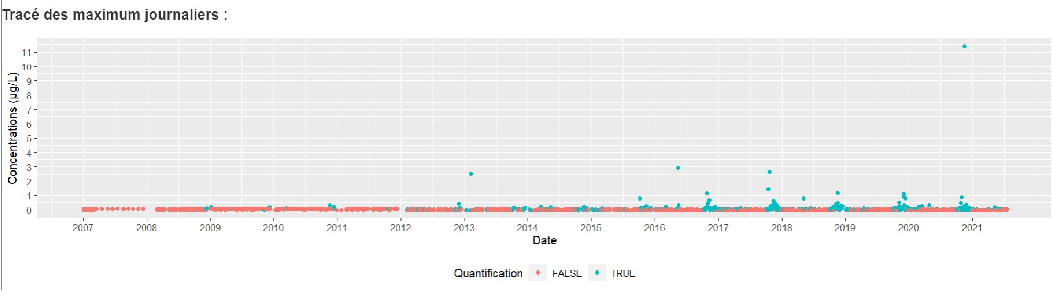
\includegraphics[]{figs/Chap6/Im_app1.pdf}
  \caption{Global temporal presentation.}
  \label{fig:Imapp1}
\end{figure}

The third element (Figure \ref{fig:Imapp2}) is the map of the stations that were active during the period study. The rivers are also represented. The stations are colored according to the station graph component they belong to. We use the same method described in Section \ref{subsection:graph:construct} relting on the BDTOPO database to create the links between stations. 

\begin{figure}[H]
  \centering
  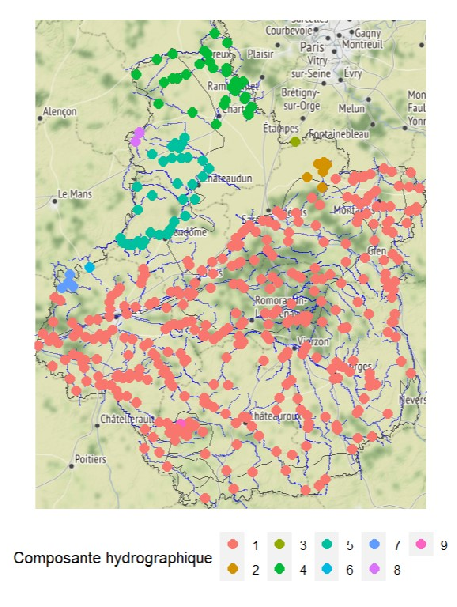
\includegraphics{figs/Chap6/Im_app2.pdf}
  \caption{Global geographical presentation.}
  \label{fig:Imapp2}
\end{figure}

\section{Detection tab}\label{chp:6:2}

We condense the results of Chapter \ref{chp:5} in this single tab. The three steps of temporal detection, spatial clustering and anomaly detection are splitted in four parts.  

\subsection{Temporal detection}\label{chp:6:2:temp}

The temporal detection is spread across two information boxes. The first box contains the segmentation performed on the daily maximum time series. Several elements are made available to the user:  
\begin{itemize}
\item Several segmentation results of the daily maximum time series are computed with the CROPS algorithm. For each segmentation, we have its corresponding penalty value. A curser to select the penalty value is displayed alongside with a graph of the different segmentations cost against their number of change points (see Figure \ref{fig:Imapp3}). For a selected penalty value in Figure \ref{fig:Imapp3}, the corresponding segmentation is highlighted in red in Figure \ref{fig:Imapp3}. The red lines are the bipartite linear models obtained using the elbow method Algorithm \ref{chp:3:algoelbow}. This provides the indication of what would be the optimal number of change-points. The application starts on the penalty value assoociated to the segmentation which cost is located on the elbow position. We selected a non optimal segmentation on purpose in the figures. 
\begin{figure}[ht]
  \centering
  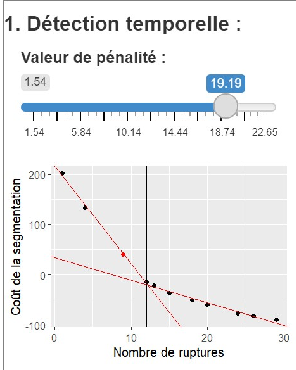
\includegraphics[]{figs/Chap6/Im_app3.pdf}
  \caption{Penalty choice and corresponding segmentation information.}
  \label{fig:Imapp3}
\end{figure}
\item Once the penalty value is set, the resulting segmentation on the daily maximum concentration signal is displayed as in Figure \ref{fig:Imapp4}. This element is reactive to the penalty value and update according to the penalty value. It is also possible to select a segment in the signal. In this case, it is highlighted in black. It is the case in Figure \ref{fig:Imapp4}. Lots of concentration values are under the quantification threshold. If some high concentration values occured in the signal, it can be complicated to distinguish low values of concentration. Hence, we added the possibility to plot the time series in logarithmic scale to obtain a better visualization. The concentrations in Figure \ref{fig:Imapp4} are plotted in logarithmic scale.  
\begin{figure}[ht]
  \centering
  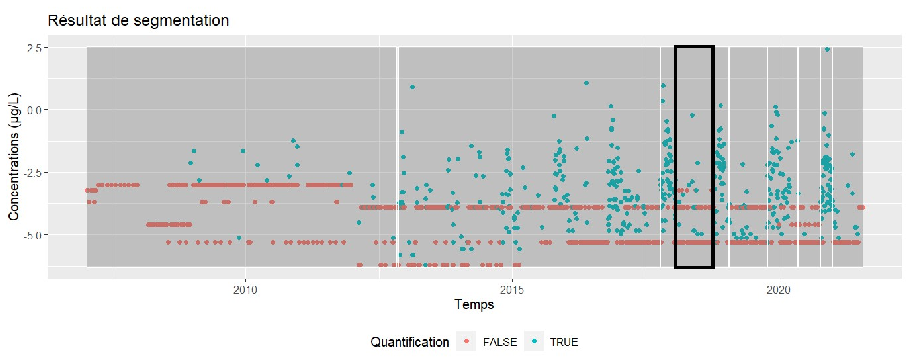
\includegraphics[]{figs/Chap6/Im_app4.pdf}
  \caption{Plot of the resulting segmentation.}
  \label{fig:Imapp4}
\end{figure}     
\end{itemize}  



The second information box is dependant of the segment selected in Figure \ref{fig:Imapp4}. Addtionnal informations specific to this segment are displayed:
\begin{itemize}
\item The following informations are given in the form of text: the dates that define the segment temporal boarders; the number of daily maximum concentration values inside the segment; the quantification percentage of the segment; the number of active stations inside the temporal period defined by the segment; the minimum, the mean, the median and the maximum values of daily maximum concentrations inside the segment. 
\item The goodness of fit is assessed by comparing the parametric cumulative distribution function to the empirical one. The plot is illustrated in Figure \ref{fig:Imapp5}, vertical black lines are drawned at the LOQ values. The empircal cdf is drawned in blue and the one obtained with the parametric model is drawned in red. Using the application confirms that the more data are present in a segment, the better the goodness of fit is. The segment selected in Figure \ref{fig:Imapp4} contained few measurments which implies the quality of the fit presented in Figure \ref{fig:Imapp5}. 
\item The last information is a seasonnal plot. When a segment is selected, we provide a comparison of the violin plot of this segment with similar time periods on the previous and following years. For instance in Figure \ref{fig:Imapp4}, the selected segment spans from the 22nd of January to the 5th of October of the year 2018. We represented the violin plot of the daily maximum concentrations from the 22nd of January to the 5th of October of each year available in Figure \ref{fig:Imapp5}. The violin plot of the selected segment is highlighted in red. Note that the violin plots adapt to whether the logarithmic scale was chosen or not in the previous information box.
\end{itemize}  

\begin{figure}[ht]
  \centering
  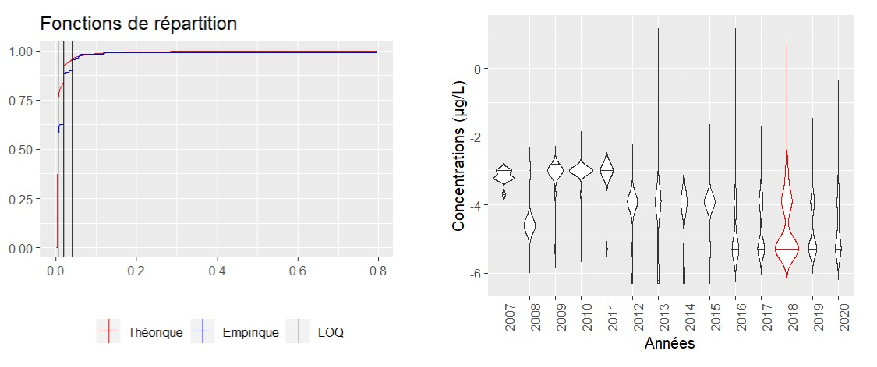
\includegraphics[]{figs/Chap6/Im_app5.pdf}
  \caption{Informations on the selected segment.}
  \label{fig:Imapp5}
\end{figure}

This two boxes encompasses the whole temporal detection procedure. The selection of the segment in Figure \ref{fig:Imapp4} determines not only the information in the second box but also all the informations that are presented in the spatial clustering and anomaly detection steps.

\subsection{Spatial clustering and anomaly detection}

Just as the temporal segmentation, the spatial clustering and the anomaly detection steps are condensed into two information boxes. The first one is a box with a map and several other elements. 

A drop-down menu is present to choose the information to display on the map. As stated previously, the information is dependant of the temporal segment selected in Section \ref{chp:6:2:temp}. The user can opt for four different options: the information of activity of a station, the stations are colored differently if they made a sample or not during the segment time period; the information of the station graph components, stations are colored according to the component they belong to in the graph of stations; the cluster information, stations are colored according to which cluster they belong to (see Figure \ref{fig:Imapp6}); the pareto front information, stations are colored according to their Pareto front level (see Figure \ref{fig:Imapp7}). The map of the graph component is redundant with the Home tab information but it was still implemented in this box as well to avoid changing tab to get that information. The graph clustering is obtained using the clustering methods presented in Algorithm \ref{algo:dyn}.  
   
Once the information is set on either the clustering information or the Pareto front levels, it is dependant on the number of cluster information. Several clustering results were imported in the application with their respective number of clusters ranging between two values. The heuristic we use to determine the minimal and maximal values of clusters in the clustering is presented in Appendix \ref{app:chap6:1}. This number can be selected with a curser located on the left in Figure \ref{fig:Imapp6} and \ref{fig:Imapp7}. The map update automatically with the number of clusters information.  

\begin{figure}[ht]
  \centering
  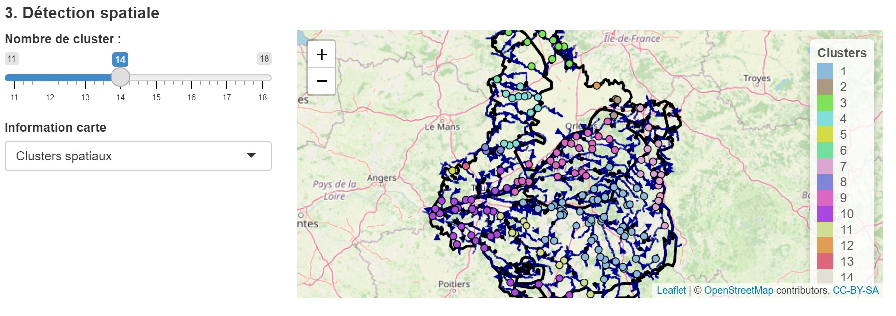
\includegraphics[]{figs/Chap6/Im_app6.pdf}
  \caption{Map displaying the clusters. The clustering selected is composed of 14 clusters.}
  \label{fig:Imapp6}
\end{figure}

\begin{figure}[ht]
  \centering
  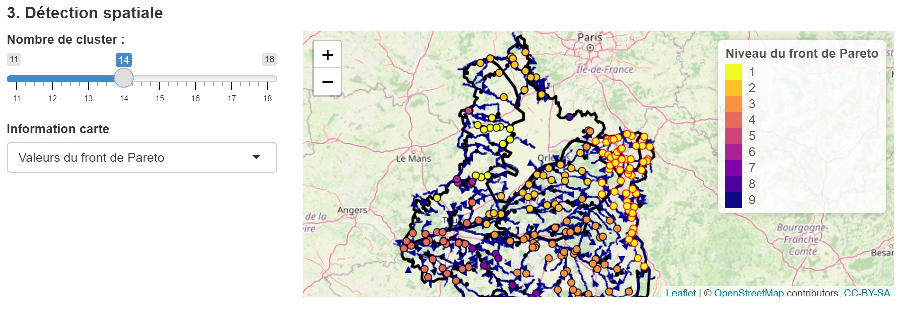
\includegraphics[]{figs/Chap6/Im_app7.pdf}
  \caption{Map displaying the Pareto front values of each cluster.}
  \label{fig:Imapp7}
\end{figure}

Additionally, there is a cluster selection feature when selecting on a station. The cluster in which the station is located is highlighted in red as in Figure \ref{fig:Imapp7}. The last box of the tab is dependnanf of this choice. The last box is composed of three windows:   
\begin{itemize}
\item The station concentration window: once a station has been selected, this window displays the samples it made during the time period of the selected segment. An illustration is provided in Figure \ref{fig:Imapp9}
\begin{figure}[ht]
 \centering
 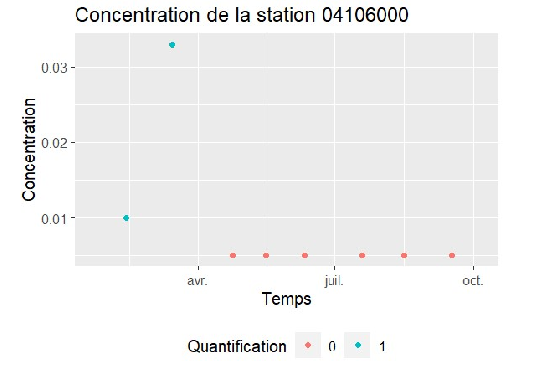
\includegraphics[]{figs/Chap6/Im_app9.pdf}
 \caption{Selected station sample values during the selected temporal segment.}
 \label{fig:Imapp9}
\end{figure}
\item The clusters Pareto plot window: clusters are plotted according to their criterion values defined in Section \ref{section:anomaly} (see Figure \ref{fig:Imapp8}). The selected cluster in the map is also highlighted in red in the plot. 
\begin{figure}[ht]
 \centering
 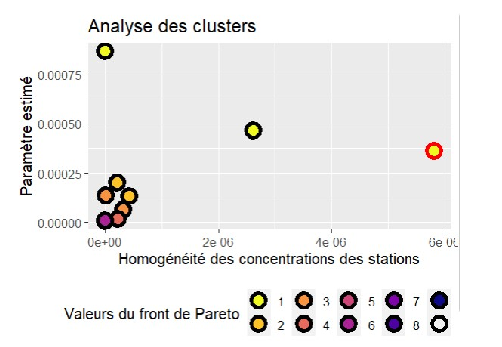
\includegraphics[]{figs/Chap6/Im_app8.pdf}
 \caption{Plot of the Pareto front.}
 \label{fig:Imapp8}
\end{figure}
\item Additionnal text informations are provided on all samples made by the stations belonging to the selected cluster in the last window such as: the total number of samples made in that cluster in the time period selected; the percentage of quantification of these samples; the number of stations composing the cluster; the minimum, the mean, the median and the maximum of concentration values in the cluster; the LOQ values present in that cluster with the information of the most frequent LOQ; the ID of the station that has the highest quantification rate with its associated percentage of quantification rate and the number of samples that were performed. The LOQ values of a cluster provide an overview of the equipment quality that is installed on the stations.    
\end{itemize}
